\begin{figure}
\centering
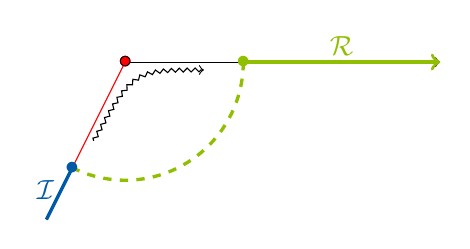
\begin{tikzpicture}[scale=1]
\draw[->] (0,2) to (2+2,2);
\draw[-,red] (0,2) to (-1,0);

\draw[->,very thick,black!25!lime] (1.5,2) to (4,2);
\node[black!25!lime] at (1.5,2) {$\bullet$};
\node at (2.75,2.2) {\textcolor{black!25!lime}{$\mathcal{R}$}};


\draw[-,very thick,black!25!lime,dashed] (1.5,2) arc (0:-117:1.5);

\draw[-,blue!30!teal,very thick] (0-0.675,2-0.675*2) to (-1,0);

\node[blue!30!teal] at (0-0.675,2-0.675*2) {$\bullet$};
\node[blue!30!teal] at (-6.5/8-0.2,0.375) {$\mathcal{I}$};

%\draw[-,black!25!lime,thick] (1.6,2.2) to (1.5,2.2) to (1.5,1.8) to (1.6,1.8);


\draw[->,decoration = {zigzag,segment length = 1mm, amplitude = 0.25mm},decorate] (0.1-0.5,1) .. controls (0+0.1,2-0.1) .. (1,1.9);
\node[rotate=180-30,scale=0.75] at (0.1-0.5,1) {$\blacktriangle$};
\node[rotate=-90,scale=0.75] at (1,1.9) {$\blacktriangle$};

\node[color=red] at (0,2) {$\bullet$};
\node[] at (0,2) {$\circ$};
\end{tikzpicture}
\caption{A cartoon depiction of the setup, with the brane in red, the bath in black, and the interface represented as a dot. The two-headed arrow indicates transparent boundary conditions. By computing the entanglement entropy of the radiation region $\mathcal{R}$, the island rule demands that we \textit{also} minimize over possible regions on the brane $\mathcal{I}$. Classically in (III), we end up with the $\mathcal{I}$ for which the entanglement surface area (possibly including brane-action contributions) is minimal.}
\label{figs:islands}
\end{figure}